
\chapter{Arbeidsmetode}
\label{app:arbeidsmetode}
I dette vedlegget beskrives det hvordan prosjektgruppen planla og satt sammen en utviklingsmetode inspirert av MVP og Scrum. Denne plannen ble satt opp helt i begynnelsen av prosjektperioden. 

\subsection{Arbeidsmetodikk}
\label{app:arbeidsmetode_arbeidsmetodikk}
Ettersom oppdraget skal ferdiggjøres på kun noen måneder er det valgt å bruke en smidig utviklingsmodell. Dette passer også godt overens med at prosjektgruppen er på kun tre personer. Produktet skal utvikles med teknologier som er ukjente både for oppdragsgiver og prosjektgruppen, derfor kan endringshyppigheten være stor under utvikling. Med en smidig utviklingsmodell kan det brukes iterasjoner for å hele tiden kunne endre på prototypen uten at det får for store konsekvenser. Fordi utviklingstiden for oppdraget er relativt kort ble det anbefalt av oppdragsgiver å bruke elementer fra Lean Startup. Derfor kommer gruppen til å bruke  Minimum Viable Product (MVP)\footnote{En versjon av produktet som dekker kundens behov og går gjennom en Lean Startup iterasjon med minst mulig bruk av ressurser og tid} og varierende iterasjoner fra Lean Startup. Varierende iterasjoner muliggjør tidlig og ofte levering av en fungerende prototype til oppdragsgiver. I tillegg vil det brukes elementer fra Scrum siden alle i gruppen er godt kjent med Scrum og oppdragsgiver bruker modellen mye i deres utviklingsprosjekter. I hovedsak kommer vi til å bruke rollene, møter og "product backlog" fra Scrum.
\\
\\
Kort oppsummert, Scrum vil bli brukt til alt rundt iterasjonene, mens selve iterasjonene vil være bygd opp av elementer fra Lean Startup.
\\
\\
Selv om utviklingen skal skje med varierende iterasjoner er det satt noen beslutningspunkter underveis i utviklingen, dette for å skape en visshet om at utviklingen går fremover. Under disse beslutningspunktene vil det holdes demomøter for oppdragsgiver. I tillegg vil det gjøres en release av prototypen til oppdragsgiver. Fordi gruppen skal utvikle en prototype og ikke et ferdig produkt vil det ikke bli gjort releaser til sluttbruker underveis.
\\
\\
Ettersom prosjektet er en del av bacheloroppgaven til gruppen kreves dokumentasjon på arbeidet som gjøres underveis. Som nevnt vil Scrum sin "product backlog" benyttes. Denne vil bestå av PBIer knyttet til user stories i kravspesifikasjonen og elementer knyttet til rapporten. For å dokumentere design og arkitekturfasen vil Rational Unified Process(RUP) sitt Software Architecture Document(SAD) bli benyttet. For å dokumentere utviklingsprosessen vil det bli skrevet møtereferater fra planleggingsmøter, vurderingsmøter, retrospektive møter og demomøter.

\pagebreak
\begin{figure}[!htbp]
    \begin{center}
        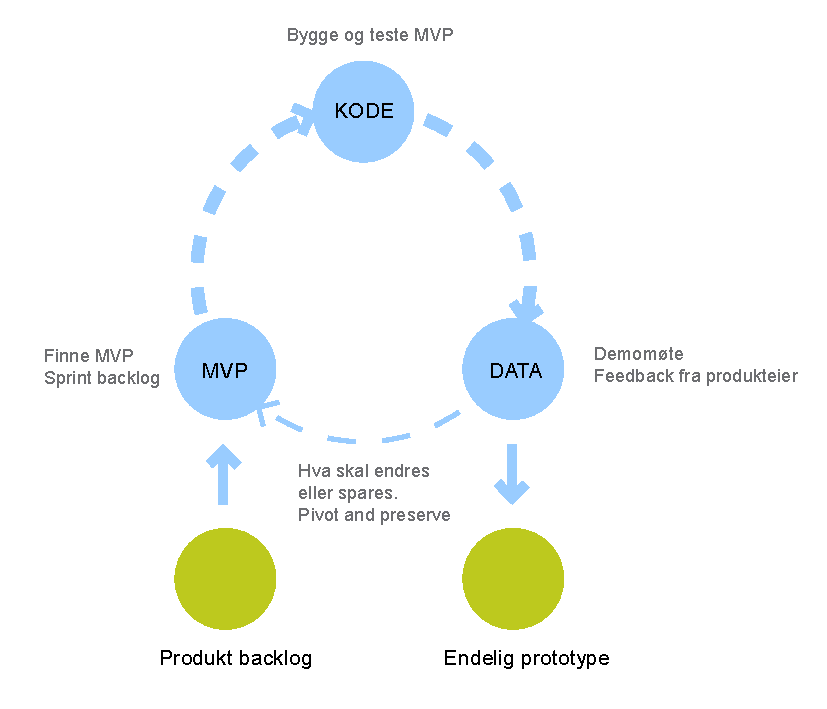
\includegraphics[scale=0.80]{graphics/UtviklingsModell}
        \caption{Utviklingsmodell for Norkart ID}
        \label{fig:utviklingsmodell}
    \end{center}
\end{figure}

\subsection{Iterasjonssirkel}
\label{app:arbeidsmetode_arbeidsmetodikk_iterasjonssirkerl}
Hver iterasjon vil bestå av sirkelen vist i figur \ref{fig:utviklingsmodell}. En iterasjon er ferdig når MVP har gått gjennom denne sirkelen. Sirklen er definert av prosjektgruppen med inspirert av "lean startup" og "Scrum".

\subsection*{MVP}
Den første fasen i iterasjonen er MVP. I denne fasen vil det holdes et planleggingsmøte hvor målet er å definere en MVP for oppkommende sprint.

\subsubsection*{KODE}
I kodefasen skal MVP utvikles og testes.

\subsubsection*{DATA}
Data er den siste fasen i en iterasjon. Her skal det holdes et gjennomgangsmøte hvor resultatet av iterasjonen presenteres for oppdragsgiver og oppdragsgiver gir så tilbakemelding. I tillegg vil det holdes et retrospektivt møte her. 
\\
\\
Etter datafasen i iterasjonen er gjort vil det holdes et endringsmøte hvor gruppen må bestemme om utviklingen kan gå videre i neste iterasjon eller om MVP må endres eller gjøres på nytt.

\subsection{Roller}
\label{app:arbeidsmetode_arbeidsmetodikk_roller}
Gruppen kommer til å bruke roller fra Scrum. Oppdragsgiver stiller med produkteier og Scrum master (omtalt som veileder), mens medlemmene i gruppa er team medlemmer.


\subsection{Møter}
\label{app:arbeidsmetode_arbeidsmetodikk_møter}
Under utvikling av Norkart ID vil det holdes en del møter. Dette blir gjort for å skape oversikt og opprettholde et godt samarbeid. I tillegg vil disse møtene brukes som dokumentering av utviklingsprosessen.

\subsection*{Planleggingsmøte}
\bigskip{}
\begin{tabular}{l p{11cm}}
    Når: & I MVP fasen \\
    Deltagere: & Gruppen \\
    Hensikt: & Fastsette en MVP og hvilke tasker som trengs for å utvikle denne i kommende sprint
\end{tabular}

\subsection*{Gjennomgangsmøte}
\bigskip{}
\begin{tabular}{l p{11cm}}
    Når: & I datafasen \\
    Deltagere: & Gruppen og oppdragsgiver \\
    Hensikt: & Presentere utviklet MVP for oppdragsgiver. Oppdragsgiver gir tilbakemelding på MVP.
\end{tabular}

\subsection*{Retrospektivtmøte}
\bigskip{}
\begin{tabular}{l p{11cm}}
    Når: & I datafasen \\
    Deltagere: & Gruppen \\
    Hensikt: & Gjennomgang av utviklingsperioden som har vært og finne eventuelle endringer som bør gjøres før neste iterasjon. Dette har til hensikt å skape overblikk over fremdrift
\end{tabular}

\subsection*{Endringsmøte}
\bigskip{}
\begin{tabular}{l p{11cm}}
    Når: & Mellom to sprinter \\
    Deltagere: & Gruppen \\
    Hensikt: & Bestemmer om utviklingen kan gå videre eller om MVP må endres eller gjøres på nytt.
\end{tabular}

\subsection*{Demomøte}
\bigskip{}
\begin{tabular}{l p{11cm}}
    Når: & Under hvert beslutningspunkt \\
    Deltagere: & Gruppen og oppdragsgiver \\
    Hensikt: & Demomøte av prototype holdes for oppdragsgiver. Oppdragsgiver får i tilleg en release av prototypen.
\end{tabular}
\bigskip{}
I tillegg til møtene nevnt ovenfor kommer gruppen til å ha møte med veiledere en gang i uken, så fremt det er nødvendig. Gruppen kommer også til benytte seg av Scrums daglige møter og det vil holdes statusmøter hver mandag.

